\documentclass[thesis.tex]{subfiles}

\begin{document}

Coupled cluster theory is based on expressing the $N$-particle correlated wave function $\corrket$ using the exponential ansatz,
\begin{equation} \label{eq:cc_ansatz}
  \corrket = \E^{\hat{T}}\refket.
\end{equation}
The cluster operator $\Top \equiv \Top_{1} + \Top_{2} + \cdots + \Top_{N}$, is composed of $k$-particle $k$-hole excitation operators, $\Top_{k}$, which have the form,
\begin{equation} \label{eq:cc_amps}
  \hat{T}_{k} \equiv \left(\frac{1}{k!}\right)^2 \sum_{\substack{a_1 \ldots a_k \\ i_1 \ldots i_k}} \tamp{a_1 \ldots a_k}{i_1 \ldots i_k}\normord{\hat{a}_{1}^\dagger \ldots \hat{a}_{k}^\dagger \hat{i}_{k}^{} \ldots \hat{i}_{1}^{}},
\end{equation}
where the unknown matrix elements, $\tamp{a_1 \ldots a_k}{i_1 \ldots i_k}$, are known as \textit{cluster amplitudes} \cite{SHAVITT2009}.

Using the CC ansatz, the Schr\"odinger equation can be rewritten by left-multiplying by $\refbra \E^{-\Top}$ as,
\begin{gather} \label{eq:cc_schrodeq}
  \Ham \E^{\Top} \refket = E \E^{\Top} \refket \notag \\
  \longrightarrow \ \ \refbra\EHam\refket = E,
\end{gather}
where we define the \textit{coupled cluster effective Hamiltonian},
\begin{align} \label{eq:cc_heff0}
  \EHam \equiv \E^{-\Top} \Ham \E^{\Top},
\end{align}
in which the wave operator, $\E^{\Top}$, acts as a similarity transform on the Hamiltonian.  An important characteristic of the effective Hamiltonian, $\EHam$, is that because the cluster operator, which contains no de-excitations, is not Hermitian, the exponential wave operator cannot be unitary, and thus $\EHam$ is not Hermitian.  This initially seems like an explicit contradiction to any standard quantum mechanics formulation where observables are associated with the real eigenvalues of Hermitian matrices. complication requires some special considerations when using coupled cluster theory, but 

The effective Hamiltonian in Eq.\ \eqref{eq:cc_heff0} can be rewritten with commutators according to the Baker--Campbell--Hausdorff expansion as,
\begin{align*}
  \EHam = \Ham + [\Ham, \Top] + \frac{1}{2!} [[\Ham, \Top], \Top] + \frac{1}{3!} [[[\Ham, \Top], \Top], \Top] + \frac{1}{4!} [[[[\Ham, \Top], \Top], \Top], \Top],
\end{align*}
which terminates at four-nested commutators due to the two-body nature of the interaction.  Like with IM-SRG, this commutator expression ensures that CC is size-extensive and contains only connected terms.  In addition, because $\Top$ is an excitation operator, terms of the form $\Top\Ham$ are disconnected and thus vanish \cite{SHAVITT2009}.  Therefore the CC effective Hamiltonian can be further reduced to
\begin{align} \label{eq:cc_heff1}
  \EHam = \left(\Ham e^{\hat{T}}\right)_{\mathrm{c}},
\end{align}
where the subscript ``$\mathrm{c}$'' indicates that only connected terms are used.

In practice, the cluster operator $\Top$ must be truncated for calculations to be computationally feasible.  In this work, we use only single and double excitations,
\begin{align*}
  \Top = \Top_{1} + \Top_{2}.
\end{align*}
This is known as coupled cluster with singles and doubles (CCSD), with an asymptotic computational cost that scales like IM-SRG(2).  This truncation has been successfully applied to many problems in quantum chemistry \cite{BARTLETT2007291} and nuclear physics \cite{HAGEN2014096302}.  In addition, we also truncate the three-body effective Hamiltonian terms that are induced by the similarity transformation.  Fig.\ \ref{fig:diagrams-ccsd} shows the diagrammatic representation of Eq.\ \eqref{eq:cc_heff1} in CCSD.

The unknown cluster amplitudes in CCSD, $\amp{a}{i}$ and $\amp{ab}{ij}$, are calculated by left-multiplying Eq.\ \eqref{eq:cc_schrodeq} by $\statebra{a}{i} \E^{-\Top}$ and $\statebra{ab}{ij} \E^{-\Top}$, respectively,
\begin{align} \label{eq:ccsd1}
  \statebra{a}{i} \EHam \refket &= 0, \\
  \statebra{ab}{ij} \EHam \refket &= 0. \notag
\end{align}
After the Fock matrix has been diagonalized, the diagonal components of Eq.\ \eqref{eq:ccsd1} can be separated and, after expanding the exponent in Eq.\ \eqref{eq:cc_heff1}, the non-vanishing terms of the CCSD amplitude equations become,
\begin{gather} \label{eq:ccsd2}
  \statebra{a}{i} \left[ \Ham_{2} \left(\Top_{1} + \Top_{2} + \Top_{1}\Top_{2} + \frac{1}{2!} \Top_{1}^{2} + \frac{1}{3!} \Top_{1}^{3}\right) \right]_{\mathrm{c}} \refket = \Edenom{a}{i}\amp{a}{i} \\
  \statebra{ab}{ij} \left[ \Ham_{2} \left(1 + \hat{T}_1 + \hat{T}_2 + \frac{1}{2} \hat{T}_1^{2} + \hat{T}_1\hat{T}_2 + \frac{1}{2!} \hat{T}_2^{2} + \frac{1}{3!} \hat{T}_1^{3} + \frac{1}{2!} \hat{T}_1^{2} \hat{T}_2 + \frac{1}{4!} \hat{T}_1^{4}\right) \right]_{\mathrm{c}} \refket = \Edenom{ab}{ij}\amp{ab}{ij} \notag
\end{gather}
where $\Edenom{}{}$ are the M\o ller--Plesset denominators from Eq.\ \eqref{eq:moellerplessetdenominator}.  As usual, these non-linear equations are solved using an iterative procedure where the cluster amplitudes on the right-hand side of Eq.\ \eqref{eq:ccsd2} are updated by calculating the terms on the left-hand side until a fixed point is reached.  Like the HF iterative procedure, employing convergence acceleration techniques can reduce the number of CC iterations required.


\section{Connection to MBPT} \label{section:linkedcluster}

The factorization theorem. (hugenholtz 1957, frantz and mills 1960, brandow 1967, 1977).
A sum over all the time orderings between a pair of disconnected diagrams is equal to the product of those two diagrams.

Linked-cluster theorem,
\begin{equation}
  \ket{\Psi^{(1)}} = \sddiagram{MBPT_linked/MBPT_linked-figure0} + \sdiagram{MBPT_linked/MBPT_linked-figure1}
\end{equation}
\begin{align}
  \ket{\Psi^{(2)}} &= \sdiagram{MBPT_linked/MBPT_linked-figure2} + \sdiagram{MBPT_linked/MBPT_linked-figure3} + \sddiagram{MBPT_linked/MBPT_linked-figure4} + \sddiagram{MBPT_linked/MBPT_linked-figure5} \notag \\
  &+ \sddiagram{MBPT_linked/MBPT_linked-figure6} + \sddiagram{MBPT_linked/MBPT_linked-figure7} + \sddiagram{MBPT_linked/MBPT_linked-figure8} + \sddiagram{MBPT_linked/MBPT_linked-figure9} + \sddiagram{MBPT_linked/MBPT_linked-figure10} \notag \\
  &+ \sddiagram{MBPT_linked/MBPT_linked-figure11} + \sddiagram{MBPT_linked/MBPT_linked-figure12} + \sdiagram{MBPT_linked/MBPT_linked-figure13} + \sdiagram{MBPT_linked/MBPT_linked-figure14} + \sdiagram{MBPT_linked/MBPT_linked-figure15} \notag \\
  &+ \sdiagram{MBPT_linked/MBPT_linked-figure16} + \sdiagram{MBPT_linked/MBPT_linked-figure17} + \sdiagram{MBPT_linked/MBPT_linked-figure18} + \sdiagram{MBPT_linked/MBPT_linked-figure19} + \sdiagram{MBPT_linked/MBPT_linked-figure20}
\end{align}



\section{Example: Pairing Model} \label{section:pairingmodel}

It's beneficial to illustrate a simplified example of coupled cluster theory.  For this purpose, we turn our attention to the simple pairing model.  This pairing model will use a model space of $N$ shells, each with two opposite spin orbitals.
\begin{figure}[h]
  \centering
  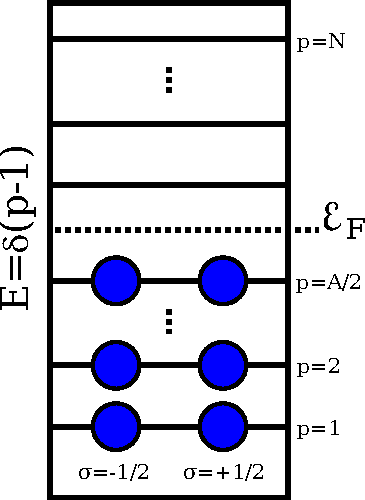
\includegraphics[width=0.35\linewidth]{CC/Pairing_Space.pdf}
  \caption{Schematic representation of the pairing model space.  The shells are equally spaced and doubly degenerate.}
  \label{fig:pairing_space}
\end{figure}

With a closed-shell reference states, the Hamiltonian is restricted to interact only between unbroken pairs, which can be written as,
\begin{gather} \label{eq:pairing_ham}
  \HamB{1} = \delta \sum_{p}^{N} \mathop{(p-1)} \left[ \co{p_{+}}\ao{p_{+}} +\ \co{p_{-}}\ao{p_{-}} \right],\ \ \text{and} \notag \\
  \HamB{2} = -\frac{g}{2} \sum_{pq}^{N} \co{p_{+}}\co{p_{-}}\ao{q_{-}}\ao{q_{+}},
\end{gather}
where $\delta$ and $g$ are free parameters and the $\pm$ labels represent the spin-up and spin-down states, respectively.

As with all other coupled cluster calculations in this work, the first step is transforming the problem to the Hartree-Fock basis.  In this case, the restriction to unbroken pairs means that the original single-particle states do not mix with states in other shells, as is generally the case from Eq.\ \eqref{eq:fock_matrix_prime}.  This means that the original basis is already an eigenbasis of the Fock operator, Eq.\ \eqref{eq:fock_operator}, so that all is left of the HF transformation is to redefine the single-particle energies to their corresponding Hartree-Fock energies while the two-body interaction is left unchanged,
\begin{gather}\label{eq:pairing_hf}
  \varepsilon_{p_{m_{p}}} = \Hint{1}{p_{m_{p}}}{p_{m_{p}}} + \sum_{im_{i}}\Hint{2}{p_{m_{p}}i_{m_{i}}}{p_{m_{p}}i_{m_{i}}} = \delta\mathop{(p-1)} - \frac{g}{2} \notag \\
  \vint{pq}{rs} = \Hint{2}{pq}{rs}
\end{gather}
Again, because of the pairing restriction, only hole-state energies have to be redefined.

The next step in calculating the ground-state correlation energy is to solve the CCD equations in the Hartree-Fock basis.  The system of equations comes from the terms of Eq.\ \eqref{eq:ccsd2} that contain only the $\Top_{2}$ operator, and are most easily derived with diagrammatic techniques, see \cite{SHAVITT2009}.
\begin{gather} \label{eq:ccd_equations}
  \statebra{ab}{ij}\mathop{(\Ham\E^{\Top_{2}})_{\text{C}}}\refket\ - \diagram{CCSD_t2/CCSD_t2-figure2} - \diagram{CCSD_t2/CCSD_t2-figure1} = \diagram{CCSD_t2/CCSD_t2-figure0} \notag \\[-1.5ex]
  + \diagram{CCSD_t2/CCSD_t2-figure5} + \diagram{CCSD_t2/CCSD_t2-figure6} + \diagram{CCSD_t2/CCSD_t2-figure7} + \diagram{CCSD_t2/CCSD_t2-figure11} \notag \\[-1.5ex]
  + \diagram{CCSD_t2/CCSD_t2-figure12} + \diagram{CCSD_t2/CCSD_t2-figure13} + \diagram{CCSD_t2/CCSD_t2-figure14} \notag \\
  \mathop{(\varepsilon_{i} + \varepsilon_{j} - \varepsilon_{a} - \varepsilon_{b})}\tamp{ab}{ij} = \vint{ab}{ij} + \frac{1}{2}\sum\limits_{\mathclap{kl}}\vint{kl}{ij}\tamp{ab}{kl} + \frac{1}{2}\sum\limits_{\mathclap{cd}}\vint{ab}{cd}\tamp{cd}{ij} - \Perm{ij|ab}\sum\limits_{\mathclap{kc}}\vint{kb}{ic}\tamp{ac}{kj} \notag \\
  + \frac{1}{4}\sum\limits_{\mathclap{klcd}}\vint{kl}{cd}\tamp{ab}{kl}\tamp{cd}{ij} + \Perm{ab}\sum\limits_{\mathclap{klcd}}\vint{kl}{cd}\tamp{ac}{lj}\tamp{bd}{ki} - \Perm{ij}\frac{1}{2}\sum\limits_{\mathclap{klcd}}\vint{kl}{cd}\tamp{ab}{lj}\tamp{cd}{ki} - \Perm{ab}\frac{1}{2}\sum\limits_{\mathclap{klcd}}\vint{kl}{cd}\tamp{db}{ij}\tamp{ca}{kl}
\end{gather}
The CCD equations are written in this particular form so that an initial guess for all the amplitudes $\tamp{ab}{ij}$ can be used to calculate the right-hand side of Eq.\ \eqref{eq:ccd_equations} and update the amplitudes on the left-hand side iteratively until the amplitudes do not change within a certain tolerance.

Lastly, the CCD correlation energy can be found with the $\Top_{2}$ term of Eq.\ \eqref{eq:cc_schrodeq}.  The only resulting term is,
\begin{equation} \label{eq:ccd_energy}
  \Ecorr_{\text{CCD}} = \refbra\mathop{(\Ham\E^{\Top_{2}})_{\text{C}}}\refket\ = \diagram{CCSD_dE/CCSD_dE-figure0}\ =\ \frac{1}{4}\sum\limits_{\mathclap{klcd}}\vint{kl}{cd}\tamp{cd}{kl}
\end{equation}
The correlation energies for a specific case, with $\delta = 1.0$, $N = 4$, and $A = 4$, were calculated for a number of different interaction strengths, $g$.  The results are shown in Fig.\ \ref{fig:pairingplot} along with the MBPT correlation energies to third (MBPT3) and fourth (MBPT4) orders for comparison.  The MBPT expressions for second and third order are,
\begin{align} \label{eq:mbpt_2_3}
  \Ecorr_{\text{MBPT2}} &= \frac{1}{4}\sum\limits_{\mathclap{ijab}}\frac{\vint{ij}{ab}\vint{ab}{ij}}{\Edenom{ab}{ij}}, \\
  \Ecorr_{\text{MBPT3}} &= \Ecorr_{\text{MBPT2}} + \frac{1}{8}\sum\limits_{\mathclap{ijabcd}}\frac{\vint{ij}{ab}\vint{ab}{cd}\vint{cd}{ij}}{\Edenom{ab}{ij}\Edenom{cd}{ij}} + \frac{1}{8}\sum\limits_{\mathclap{ijklab}}\frac{\vint{ij}{ab}\vint{kl}{ij}\vint{ab}{kl}}{\Edenom{ab}{ij}\Edenom{ab}{kl}} - \sum\limits_{\mathclap{ijkabc}}\frac{\vint{ij}{ab}\vint{kb}{ic}\vint{ac}{kj}}{\Edenom{ab}{ij}\Edenom{ac}{kj}}.
\end{align}
The fourth-order expression contains 39 additional terms, so the expression for MBPT4 is omitted.
\begin{figure}[h]
  \centering
  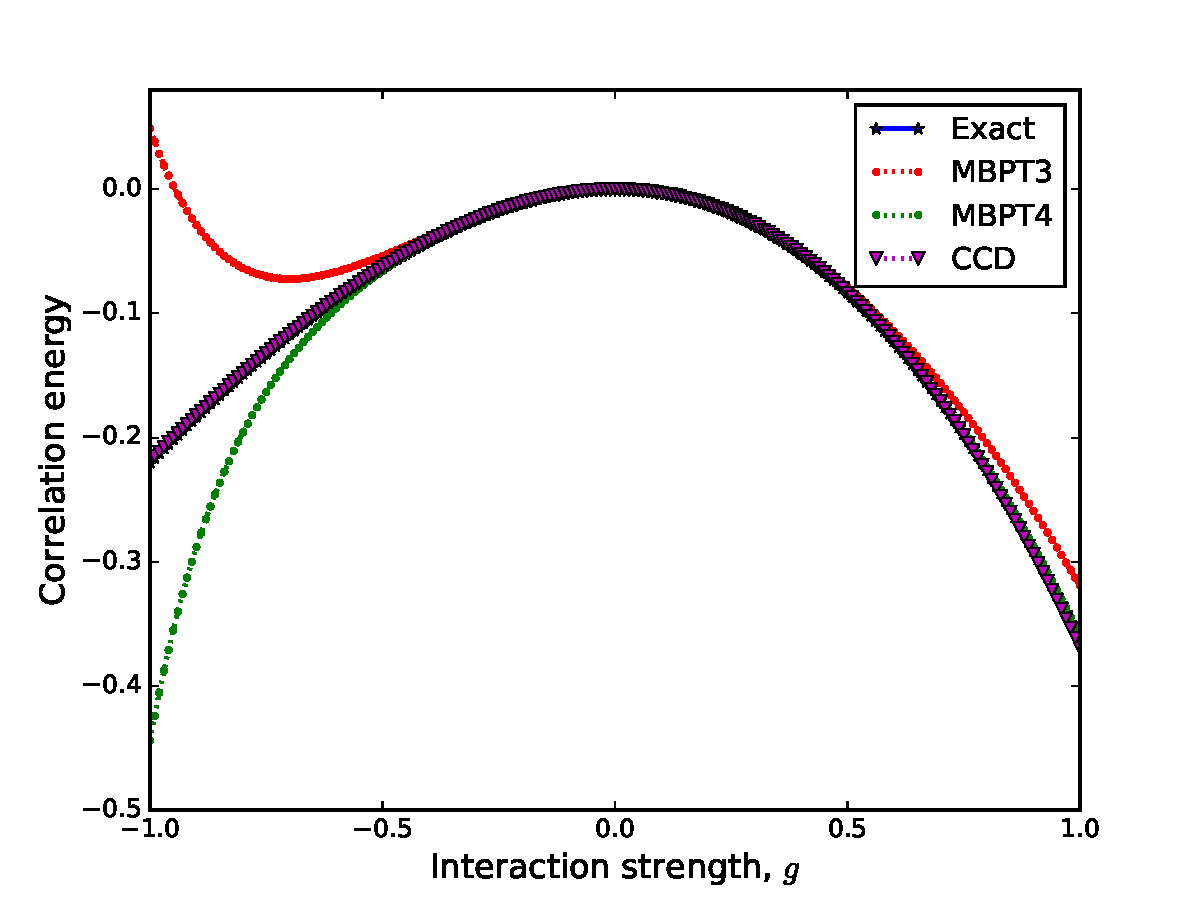
\includegraphics[width=\textwidth]{CC/CCDMBPT4theory.pdf}
  \caption{Correlation energy for the pairing model with exact diagonalization, CCD and perturbation theory to third  (MBPT3) and fourth order (MBPT4) for a range of interaction values.}
  \label{fig:pairingplot}
\end{figure}

Also shown are the exact results from the CI method.  With an example this small, it's possible to diagonalize, and even show explicitly, the full CI Hamiltonian matrix for an exact result.  The dimension of this matrix with no broken pairs accounts to six possible Slater determinants, one representing the reference state, four representing various $\ph{2}{2}$ excitations, one representing a $\ph{4}{4}$ excitation.  The diagonal elements of the matrix include the single-particle energies of the constituent states, and the matrix elements between Slater determinants with no overlap vanish in accordance with the Slater-Condon rules, see Eq.\ \eqref{eq:slater_condon} and \cite{SLATER1929,CONDON1930}.
\begin{equation}
  H = \begin{bmatrix}
    2\delta -g & -g/2 & -g/2 & -g/2 & -g/2 & 0 \\ -g/2 & 4\delta -g &
    -g/2 & -g/2 & -0 & -g/2 \\ -g/2 & -g/2 & 6\delta -g & 0 & -g/2 &
    -g/2 \\ -g/2 & -g/2 & 0 & 6\delta-g & -g/2 & -g/2 \\ -g/2 & 0 & -g/2
    & -g/2 & 8\delta-g & -g/2 \\ 0 & -g/2 & -g/2 & -g/2 & -g/2 &
    10\delta -g
  \end{bmatrix}
\end{equation}

As methods to obtain the ground-state correlation energy, both CI and CC decouple, to some degree, the reference state and excitations from it.  This decoupling has the effect of shuffling correlations into the reference state.  Full decoupling between the reference state and all other Slater determinants can only be achieved with untruncated versions of the techniques, while decoupling of the strongest correlations can be approximately obtained with appropriate truncations.  However, unlike other many-body methods, the most unique aspect of the CC similarity transformation is that because of its non-unitarity, the resulting Hamiltonian will not be Hermitian.  This decoupling and non-Hermiticity can be seen in Fig.\ \ref{fig:pairingmatrix}, which shows the effect of the CC similarity transformation on the Hamiltonian for a pairing case with $N = 6$ and $A = 4$.
\begin{figure}[h]
  \centering
  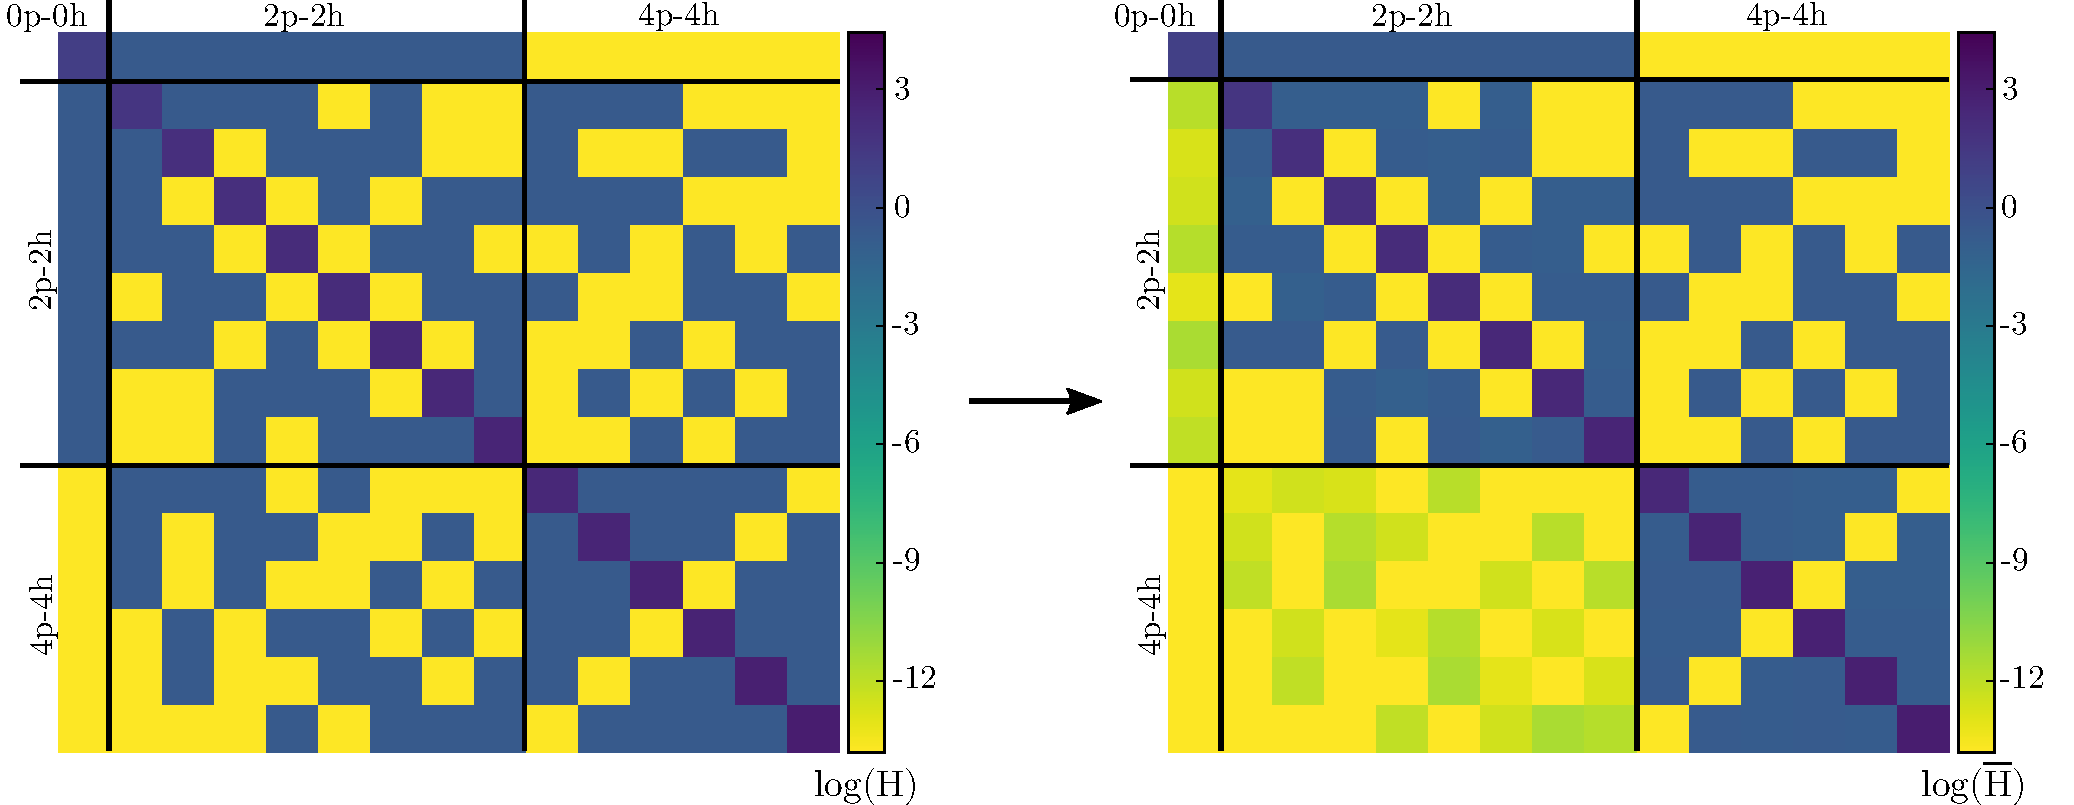
\includegraphics[width=\textwidth]{CC/pairingmatrix.pdf}
  \caption{Visualization of the CCD similarity transform on the pairing Hamiltonian for four particles and six shells.  This shows the main function of CCD, which is to decouple $\ph{2}{2}$ excitations from the ground state, shown by the suppression of matrix elements on the first column. In the pairing model, this also has the effect of decoupling $\ph{2}{2}$ excitations from $\ph{4}{4}$ excitations.  Also, the non-unitary nature of the transformation is obvious given the asymmetry of the resulting Hamiltonian.}
  \label{fig:pairingmatrix}
\end{figure}
The effective Hamiltonian $\EHam$ shown in Fig.\ \ref{fig:pairingmatrix} can be explicitly built, and it happens to be beneficial to do so as part of most CC calculations, both for solving the CC equations and for use in post-CC methods.  This topic is discussed in detail in the next section.




\section{Solving the Coupled Cluster Equations} \label{section:solvingcc}

As described above, the coupled cluster equations are solved by first initializing all of the cluster amplitudes, then updating them by computing various sums over particle and hole combinations, $\text{CC}\mathop{(\Top)}$.  This updating procedure is performed over multiple iterations until the amplitudes stay unchanged within a certain tolerance.
\begin{align} \label{eq:cc_algorithm}
  &\text{Initialize}:&    \hspace{-20pt}&\Top^{\mathop{(0)}} = \Top_{\text{init}} \notag \\
  &\text{Iterate}:&       \hspace{-20pt}&\Top^{\mathop{(n+1)}}\ \leftarrow\ \text{CC}\mathop{(\Top^{\mathop{(n)}})}
\end{align}
While the scaling of these sums are more managable than other methods, any available computing power will be used to calculate larger systems in larger bases.  Therefore, it's essential to find the most efficient way of solving a problem regardless of the problem itself.

For the coupled cluster equations, as well as many other many-body methods, the first way to simplify the various sums is to exploit any symmetries of the underlying Hamiltonian of a particular problem.  These symmetries manifest as conserved quantities.  And because of the underlying nature of the cluster operators, see Section\ \ref{section:linkedcluster}, these must conserve these quantum numbers as well.  For example, the pairing Hamiltonian of Section\ \ref{section:pairingmodel} has a symmetry that conserves both the total spin projection and the number of pairs.  The Coulomb Hamiltonian of Section\ \ref{section:electrongas}, which has spherical symmetry, conserves both the linear momentum and the angular momentum of a certain state.  Finally, the spherical symmetry of the nuclear Hamiltonian also ensures that angular momentum is conserved, along with parity.  To utilize these symmetries, any sums that contain many-body states with different conserved quantum numbers can be ignored.  For efficiency, these symmetry groups can be pre-sorted into \textit{channels}, $\Sigma_{\vec{\xi}}$, where $\vec{\xi}$ represents the relevant quantum numbers of a certain channel.

For CCSD calculations, useful types of channels include the direct two-body channels, $\Sigma_{\vec{\xi}_{1}}$--which categorizes the vector sum of two single-particle-state quantum numbers--and the cross two-body channels, $\Sigma_{\vec{\xi}_{2}}$--which categorizes the vector difference of two single-particle-state quantum numbers or, equivalently, the vector sum of a the quantum numbers of a single-particle state and a time-reversed single-particle state.
\begin{gather}
  \vec{\xi}_{pq} = \vec{\xi}_{p} + \vec{\xi}_{q}\ \ \longrightarrow\ \ \ket{pq} \in \Sigma_{\vec{\xi}_{1}=\vec{\xi}_{pq}} \\
  \vec{\xi}_{p\bar{q}} = \vec{\xi}_{p} - \vec{\xi}_{q} = \vec{\xi}_{p} + \vec{\xi}_{\bar{q}}\ \ \longrightarrow\ \ \ket{p\bar{q}} \in \Sigma_{\vec{\xi}_{2}=\vec{\xi}_{p\bar{q}}}
\end{gather}
Also useful is the one-body channels, $\Sigma_{\vec{\xi}_{3}}$, which categorizes both single-particle states by their conserved quantum numbers.  These one-body channels can also characterize a special type of three-body state, the vector difference between the qunatum numbers of a direct two-body state and a single-particle state or, equivalently, the vector sum of the quantum numbers of a two-body direct state and a time-reversed single-particle state.
\begin{gather}
  \vec{\xi}_{p}\ \ \longrightarrow\ \ \ket{p} \in \Sigma_{\vec{\xi}_{3}=\vec{\xi}_{p}} \\
  \vec{\xi}_{pq\bar{r}} = \vec{\xi}_{p} + \vec{\xi}_{q} - \vec{\xi}_{r} = \vec{\xi}_{p} + \vec{\xi}_{q} + \vec{\xi}_{\bar{r}}\ \ \longrightarrow\ \ \ket{pq\bar{r}} \in \Sigma_{\vec{\xi}_{3}=\vec{\xi}_{pq\bar{r}}}
\end{gather}

Using these channel structures, the interaction matrix elements and cluster amplitudes can be built in different ways.  The full applicability of these structures are shown in detail in chapter \ref{chapter:appendix_computational}, but a few examples using sums in the CCD equations \eqref{eq:ccd_equations} are shown here.
\begin{gather} \label{eq:channel_sums}
  \frac{1}{2}\sum\limits_{\mathclap{cd}}\vint{ab}{cd}\tamp{cd}{ij} = \frac{1}{2}\sum\limits_{\mathclap{\ket{cd}}}\vint{ab}{cd}\tamp{cd}{ij}\ \ \text{for}\ \ket{cd} \in \Sigma_{\vec{\xi}_{ab}}=\Sigma_{\vec{\xi}_{ij}} \notag \\
  \sum\limits_{\mathclap{kc}}\vint{kb}{ic}\tamp{ac}{kj} = \sum\limits_{\mathclap{\ket{k\bar{c}}}}\vint{k\bar{c}}{i\bar{b}}\tamp{a\bar{j}}{k\bar{c}}\ \ \text{for}\ \ket{k\bar{c}} \in \Sigma_{\vec{\xi}_{i\bar{b}}}=\Sigma_{\vec{\xi}_{a\bar{j}}} \notag \\
  \frac{1}{2}\sum\limits_{\mathclap{klcd}}\vint{kl}{cd}\tamp{db}{ij}\tamp{ca}{kl} = \frac{1}{2}\sum\limits_{\mathclap{\substack{\ket{kl\bar{c}} \\ \ket{d}}}}\vint{kl\bar{c}}{d}\tamp{d}{ij\bar{b}}\tamp{a}{kl\bar{c}}\ \ \text{for}\ \ket{kl\bar{c}},\ket{d} \in \Sigma_{\vec{\xi}_{ij\bar{b}}}=\Sigma_{\vec{\xi}_{a}}
\end{gather}

Symmetry channels not only provide an organization to the interaction matrix elements and cluster amplitudes and remove any terms that violate the underlying symmetry of a problem, but they also naturally provide an efficient way of performing sums using matrix-matrix multiplications.  For example, the sums in Eq.\ \eqref{eq:channel_sums} can be reformulated as matrix-matrix multiplications by structuring the channel-separated interaction matrix elements and cluster amplitudes into individual matrices.  The matrices can be reordered so that the summed indices correspond to the internal columns and rows of those matrices.
\begin{gather} \label{eq:channel_matrices}
  \frac{1}{2}\sum\limits_{\mathclap{cd}}\vint{ab}{cd}\tamp{cd}{ij} = \frac{1}{2}\bvint{ab}{cd}\cdot\btamp{cd}{ij}\ \ \text{for}\ \ket{ab},\ket{ij},\ket{cd} \in \Sigma_{\vec{\xi}_{1}} \notag \\
  \sum\limits_{\mathclap{kc}}\vint{kb}{ic}\tamp{ac}{kj} = \btamp{a\bar{j}}{k\bar{c}}\cdot\bvint{k\bar{c}}{i\bar{b}}\ \ \text{for}\ \ket{a\bar{j}},\ket{i\bar{b}},\ket{k\bar{c}} \in \Sigma_{\vec{\xi}_{2}} \notag \\
  \frac{1}{2}\sum\limits_{\mathclap{klcd}}\vint{kl}{cd}\tamp{db}{ij}\tamp{ca}{kl} = \frac{1}{2}\btamp{a}{kl\bar{c}}\cdot\bvint{kl\bar{c}}{d}\cdot\btamp{d}{ij\bar{b}}\ \ \text{for}\ \ket{a},\ket{ij\bar{b}},\ket{kl\bar{c}},\ket{d} \in \Sigma_{\vec{\xi}_{3}}
\end{gather}
These sums correspond to different components of the updated cluster amplitudes according to Eq.\ \eqref{eq:cc_algorithm}.  So the different channel structures of the matrix-matrix multiplications in Eq.\ \eqref{eq:channel_matrices} correspond to different amplitude structures according to the sums external indices.
\begin{gather} \label{eq:amp_matrices}
  \btamp{ab}{ij}\ \leftarrow\ \frac{1}{2}\bvint{ab}{cd}\cdot\btamp{cd}{ij}\ \ \text{for}\ \ket{ab},\ket{ij},\ket{cd} \in \Sigma_{\vec{\xi}_{1}} \notag \\
  \btamp{a\bar{j}}{i\bar{b}}\ \leftarrow\ \btamp{a\bar{j}}{k\bar{c}}\cdot\bvint{k\bar{c}}{i\bar{b}}\ \ \text{for}\ \ket{a\bar{j}},\ket{i\bar{b}},\ket{k\bar{c}} \in \Sigma_{\vec{\xi}_{2}} \notag \\
  \btamp{a}{ij\bar{b}}\ \leftarrow\ \frac{1}{2}\btamp{a}{kl\bar{c}}\cdot\bvint{kl\bar{c}}{d}\cdot\btamp{d}{ij\bar{b}}\ \ \text{for}\ \ket{a},\ket{ij\bar{b}},\ket{kl\bar{c}},\ket{d} \in \Sigma_{\vec{\xi}_{3}}
\end{gather}

The last summation in the matrix-matrix form of Eqs.\ \eqref{eq:channel_matrices,eq:amp_matrices} involves two multiplications, which suggests the need for an \textit{intermediate} matrix to hold the result of the first.  This is the last component to an efficient CC algorithm.  To see the benefit of intermediate structures, it's helpful to examine the most expensive sum from the CCD equations.  Because for typical calculations, particle states outnumber hole states by an order of magnitude, $N_{p} \sim 10N_{h}$, one of the most expensive sums is,
\begin{equation}
  \frac{1}{4}\sum\limits_{\mathclap{klcd}}\vint{kl}{cd}\tamp{ab}{kl}\tamp{cd}{ij}.
\end{equation}
Because this term must be computed for each $\tamp{ab}{ij}$, its computational cost naively scales as $\sim N_{h}^{4}N_{p}^{4}$.  However, using matrix form of this sum and an intermediate matrix,
\begin{equation} \label{eq:intermediate}
  \frac{1}{4}\sum\limits_{\mathclap{klcd}}\vint{kl}{cd}\tamp{ab}{kl}\tamp{cd}{ij} = \frac{1}{4}\btamp{ab}{kl}\cdot\left(\bvint{kl}{cd}\cdot\btamp{cd}{ij}\right) = \frac{1}{4}\btamp{ab}{kl}\cdot\bxint{kl}{ij}\ \rightarrow\ \btamp{ab}{ij}.
\end{equation}
Using the intermediate structure, this term is now computed as the combination of two sums, each scaling as $\sim N_{h}^{4}N_{p}^{2}$.  These intermediates can also be used as a way to combine similar sums.  For example, the last step of Eq.\ \ref{eq:intermediate} has a very similar structure to the first sum in Eq.\ \ref{eq:ccd_equations}.  Therefore, the two sums can be written with a common intermediate as,
\begin{gather}
  \frac{1}{2}\sum\limits_{\mathclap{kl}}\vint{kl}{ij}\tamp{ab}{kl} + \frac{1}{4}\sum\limits_{\mathclap{klcd}}\vint{kl}{cd}\tamp{ab}{kl}\tamp{cd}{ij} = \frac{1}{2}\btamp{ab}{kl}\cdot\left[ \bvint{kl}{ij} + \frac{1}{2}\bvint{kl}{cd}\cdot\btamp{cd}{ij} \right] = \frac{1}{4}\btamp{ab}{kl}\cdot\bxint{kl}{ij}\ \rightarrow\ \btamp{ab}{ij}, \notag \\
  \text{where},\hspace{10pt} \bxint{kl}{ij} = \bvint{kl}{ij} + \frac{1}{2}\bvint{kl}{cd}\cdot\btamp{cd}{ij}
\end{gather}

It just so happens that this form of the intermediate $\xint{kl}{ij}$ is equivalent to the $hhhh$ component of the similarity transformed Hamiltonian, $EHam$, within CCD.  Because constructing other intermediates in this way gives similar results, it's natural extension to actually construct the effective Hamiltonian for the express purpose of using the different intermediate components of the CC equations.  This has the added benefit of having already computed the effective Hamiltonian for post-CC methods.  The construction of the various components of the effective Hamiltonian, $\xint{}{}$, can also be improved with the use of various intermediates, but special terms must be used to avoid double counting diagrams, $\xxint{}{}, \xxxint{}{}, \xxxxint{}{}$.  For the CCSD effective Hamiltonian, $\EHam_{\text{CCSD}} = \left(\Ham\E^{\left(\Top_{1} + \Top_{2}\right)}\right)_{\mathrm{c}}$, the different components and intermediats are,
%%%%%%%%%%%%%%%%%%%%%%%%%%%%%%%%%%%%%%%%%%%%%%%%%%%%%%%%%%%%%%%%%%%%%%%%%%%%%%%%%%%
\begin{align} \label{eq:ccd_eff1}
  \diagram{CCSD_1b/CCSD_1b-figure3} &= \diagram{CCSD_1b/CCSD_1b-figure4} + \diagram{CCSD_1b/CCSD_1b-figure5} \notag \\
  \xint{a}{b} &= \fint{a}{b} - \frac{1}{2}\sum\limits_{klc}\vint{kl}{bc}\tamp{ac}{kl}
\end{align}
\begin{align} \label{eq:ccd_eff2}
  \diagram{CCSD_1b/CCSD_1b-figure12} &= \diagram{CCSD_1b/CCSD_1b-figure9} + \diagram{CCSD_1b/CCSD_1b-figure10} \notag \\
  \xint{i}{j} &= \fint{i}{j} + \frac{1}{2}\sum\limits_{kcd}\vint{ik}{cd}\tamp{cd}{jk}
\end{align}
\begin{align} \label{eq:ccd_eff3}
  \diagram{CCSD_2b/CCSD_2b-figure18} &= \diagram{CCSD_2b/CCSD_2b-figure19} + \diagram{CCSD_2b/CCSD_2b-figure20} \notag \\
  \xint{ij}{kl} &= \vint{ij}{kl} + \frac{1}{2}\sum\limits_{cd}\vint{ij}{cd}\tamp{cd}{kl}
\end{align}
\begin{align} \label{eq:ccd_eff4}
  \diagram{CCSD_2b/CCSD_2b-figure34} &= \diagram{CCSD_2b/CCSD_2b-figure31} + \frac{1}{2}\fdiagram{CCSD_2b/CCSD_2b-figure36} \notag \\
  \xint{ia}{jb} &= \vint{ia}{jb} - \frac{1}{2}\sum\limits_{kc}\vint{ik}{cb}\tamp{ca}{jk}
\end{align}

Using these terms, the CCSD equations can be written in pseudo-linear form.  These also explicitly show the decoupling of the effective Hamiltonian with $\ph{1}{1}$ and $\ph{2}{2}$ excitations,
\begin{align} \label{eq:ccd_double_linear}
  \diagram{CCSD_2b/CCSD_2b-figure59} = 0 &= \diagram{CCSD_2b/CCSD_2b-figure60} + \diagram{CCSD_2b/CCSD_2b-figure61} + \diagram{CCSD_2b/CCSD_2b-figure62} \notag \\[-1.5ex]
  &+ \diagram{CCSD_t2/CCSD_t2-figure6} + \diagram{CCSD_2b/CCSD_2b-figure64} + \diagram{CCSD_2b/CCSD_2b-figure65} \notag \\
  \xint{ab}{ij} = 0 &= \vint{ab}{ij} + \Perm{ab}\sum\limits_{\mathclap{c}}\xint{a}{c}\tamp{cb}{ij} - \Perm{ij}\sum\limits_{\mathclap{k}}\xint{k}{i}\tamp{ab}{kj} \notag \\
  &+ \frac{1}{2}\sum\limits_{\mathclap{cd}}\xxint{ab}{cd}\tamp{cd}{ij} + \frac{1}{2}\sum\limits_{\mathclap{kl}}\xint{kl}{ij}\tamp{ab}{kl} - \Perm{ab|ij}\sum\limits_{\mathclap{kc}}\xint{kb}{ic}\tamp{ac}{kj}
\end{align}

%-----------------


\section{Example: Infinite Matter} \label{section:infinitematter}

Another relatively simple example calculation using coupled cluster theory is that of the homogeneous electron gas.  This example aims to calculate the ground state energy of a three-dimensional gas of electrons subject to Coulomb repulsion.  This is an approximate model of the valence electrons in a metal, subject to a uniform background of positive charge from the nuclei and core electrons.  As will be explained below, this calculation employs pure-momentum eigenstates such that $\ph{1}{1}$ excitations from the reference state are forbidden by momentum conservation.  This again reduces the problem to the doubles approximation, CCD.  However, to obtain realistic reslults, a sufficiently-sized basis and a sufficient number of electrons must be used.  Thus the improvements discussed in Section \ref{section:solvingcc} will improve the speed of the calculation as its size increases.

With a uniform background potential, the electron gas can be constructed using eigenfunctions of the kinetic energy operator, $\HamB{1} = \frac{-\hbar^{2}}{2m}\nabla^{2}$.  In an infinite volume, however, there are an unlistable number of many plane wave modes which satisfy this condition, due to the continuous nature of the linear momentum eigenstates.  Therefore, the single-particle orbits will be constructed in a finite box of volume $\Omega$ and length $L$, and then the limit $L\rightarrow \infty$ can be taken after various expectation values have been computed.
\begin{gather} \label{eq:plane_wave}
  \frac{-\hbar^{2}}{2m}\nabla^{2}\phi_{\mathbf{k}\sigma}(\mathbf{r}) = \epsilon_{\mathbf{k}}\phi_{\mathbf{k}\sigma}(\mathbf{r}) \notag \\
  \phi_{\mathbf{k}\sigma}(\mathbf{r}) = \frac{1}{\sqrt{\Omega}}\exp{(i\mathbf{kr})}\xi_{\sigma}
\end{gather}
where $m$ is the electron mass, $\mathbf{k}$ is the wave number, and $\xi_{\sigma}$ is the spin function for either spin up or down electrons
\begin{equation}
  \xi_{\sigma=+1/2} = \left(\begin{array}{c} 1
    \\ 0 \end{array}\right) \hspace{0.5cm}
  \xi_{\sigma=-1/2} = \left(\begin{array}{c} 0 \\ 1 \end{array}\right).
\end{equation}

Assuming the single-particle orbits follow periodic boundary conditions within the containing box ($\phi(\mathbf{r}_{i}) = \phi(\mathbf{r}_{i} + L)$ for $i = x,y,z$) the wave numbers will be quantized to
\begin{equation}
  k_{i} = \frac{2\pi n_{i}}{L}\hspace{0.5cm} i = x,y,z \hspace{0.5cm} n_{i} = 0, \pm 1, \pm 2, \dots
\end{equation}
A state can therefore be characterized by the quantum numbers $n_{x}$, $n_{x}$, and $n_{x}$ as well as the spin qunatum number $\sigma$.  The energy of such a state, independent of the spin, can be written as
\begin{equation} \label{eq:infinite_energy}
  \epsilon_{n_{x}, n_{y}, n_{z}} = \frac{\hbar^2}{2m}\left(k_{x}^{2} + k_{y}^{2} + k_{z}^{2}\right) = \frac{\hbar^{2}}{2m}\left(\frac{2\pi }{L}\right)^{2} \left( n_{x}^{2} + n_{y}^{2} + n_{z}^{2}\right).
\end{equation}
\begin{figure}[h]
  \centering
  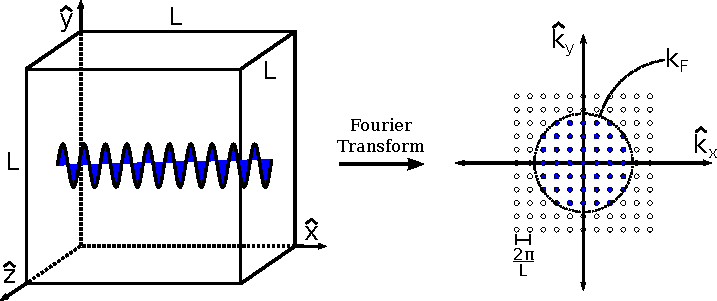
\includegraphics[width=\linewidth]{CC/Infinite_Space.pdf}
  \caption{Visulization of the Fourier transfrom of a finite box.  This transfrom characterizes the construction of the single-particle basis for infinite matter, mapping plane waves in corrdinate space onto finitely-spaced points in momentum space.}
  \label{fig:infinite_space}
\end{figure}

Now that the single-particle orbits are established, a particular basis consisting of these orbits can be chosen such that all states are included up to a closed shell.  This basis is then filled with electrons until a closed Fermi level is obtained.  Additionally, only the unpolarized case, in which all orbitals are occupied with one spin-up and one spin-down electron, will be considered here.  For this \textit{spherical} level structure, the number of electrons required for closed shells increases quickly.  For example, the first six shells contain $2$, $14$, $38$, $54$, $66$ and $114$ states, respectively.

A finite number of electrons $A$ in a finite box of volume $\Omega$ leads naturally to the characterization of an infite system by its number density density $\rho = A/\Omega$.  The average inter-electron distance, or \textit{Wigner-Seitz radius}, is defined as
\begin{equation} \label{wigner-seitz}
  \frac{4}{3}\pi r_{s}^{3} = \frac{1}{\rho},\hspace{0.5cm} r_{s} = \left(\frac{3}{4\pi\rho}\right)^{1/3}.
\end{equation}
In practice, a calculation of this time is defined by the total number of shells included in the basis, the number of electrons, and the Wigner-Seitz radius, usually given in units of the Bohr radius, $r_{b} = \frac{\hbar}{mc\alpha}$, where $c$ is the speed of light and $\alpha$ is the fine-structure constant.

The last ingredient to this many-body calculation is the interaction between the electrons, the well-known Coulomb force.  Using atomic units, where the elementary charge $e = 1$ and the Coulomb constant $\frac{1}{4\pi\varepsilon_{0}} = 1$, this potential is simply
\begin{equation} \label{eq:coulomb}
  V\left( \mathbf{r}_{1}, \mathbf{r}_{2}\right) = \frac{1}{\lvert \mathbf{r}_{1} - \mathbf{r}_{2} \rvert}.
\end{equation}
As mentioned in chapter \ref{chapter:manybody}, this potential can be utilized in second-quantization by computing antisymmetrized integrals over the basis states.  In this case, the integrals have the form,
\begin{equation} \label{eq:coloumb_integral}
  \Hint{2}{pq}{rs} \equiv \int d\mathbf{r}_{1} d\mathbf{r}_{2}\  \phi^{*}_{\mathbf{k}_{p}\sigma_{p}}(\mathbf{r}_{1})\phi^{*}_{\mathbf{k}_{q}\sigma_{q}}(\mathbf{r}_{2}) \frac{1}{\lvert \mathbf{r}_{1} - \mathbf{r}_{2} \rvert} \left[\phi_{\mathbf{k}_{r}\sigma_{r}}(\mathbf{r}_{1})\phi_{\mathbf{k}_{s}\sigma_{s}}(\mathbf{r}_{2}) - \phi_{\mathbf{k}_{s}\sigma_{s}}(\mathbf{r}_{1})\phi_{\mathbf{k}_{r}\sigma_{r}}(\mathbf{r}_{2})\right].
\end{equation}
The symmetries of the Coulomb potential guarantee that the total linear momentum and total spin projection is conserved such that,
\begin{equation} \label{eq:coulomb-conserve}
  \mathbf{k}_{p} + \mathbf{k}_{q} = \mathbf{k}_{r} + \mathbf{k}_{s} \hspace{0.5cm} \text{and} \hspace{0.5cm} \sigma_{p} + \sigma_{q} = \sigma_{r} + \sigma_{s}.
\end{equation}
The integral is relatively simple given the form of the basis functions. The result is given in terms of the momentum transfer, $\mathbf{q}_{1} = \mathbf{k}_{p} - \mathbf{k}_{r}$ and $\mathbf{q}_{2} = \mathbf{k}_{p} - \mathbf{k}_{r}$,
\begin{equation} \label{eq:coulomb-int}
  \Hint{2}{pq}{rs} = \frac{4\pi \hbar c \alpha}{\Omega}\left[ \frac{\delta_{\sigma_{p}\sigma_{r}}\delta_{\sigma_{q}\sigma_{s}}}{\lvert \mathbf{q}_{1} \rvert^{2}} - \frac{\delta_{\sigma_{p}\sigma_{s}}\delta_{\sigma_{q}\sigma_{r}}}{\lvert \mathbf{q}_{2} \rvert^{2}} \right]
\end{equation}

The last preparation step before performing the coupled cluster algorithm is the Hartree-Fock transformation.  As with the pairing model, the single-particle orbitals are already eigenfunctions of the Fock operator, and thus only the hole-state single-particle energies need to be redefined while the two-body interaction is left unchanged.
\begin{gather}\label{eq:infinite_hf}
  \varepsilon_{p} = \epsilon_{\mathbf{k}_{p}} + \sum_{i}\Hint{2}{pi}{pi} \notag \\
  \vint{pq}{rs} = \Hint{2}{pq}{rs}
\end{gather}

As metioned above, in the plane-wave basis, any single excitation from the reference state vanishes automatically due to momentum conservation, $\tamp{a}{i} = 0$.  Therefore, it's neccessary to include double excitations with CCD only (before adding expensive triples, etc.).  Using the psudo-linear form of the doubles equation \eqref{eq:double_linear} and an effective Hamiltonian that excludes single excitations in Eqns.\ \eqref{eq:eff1}.  The total energy per electron can now be calculated and plotted as a function of the Wigner-Seitz radius.
\begin{figure}[h]
  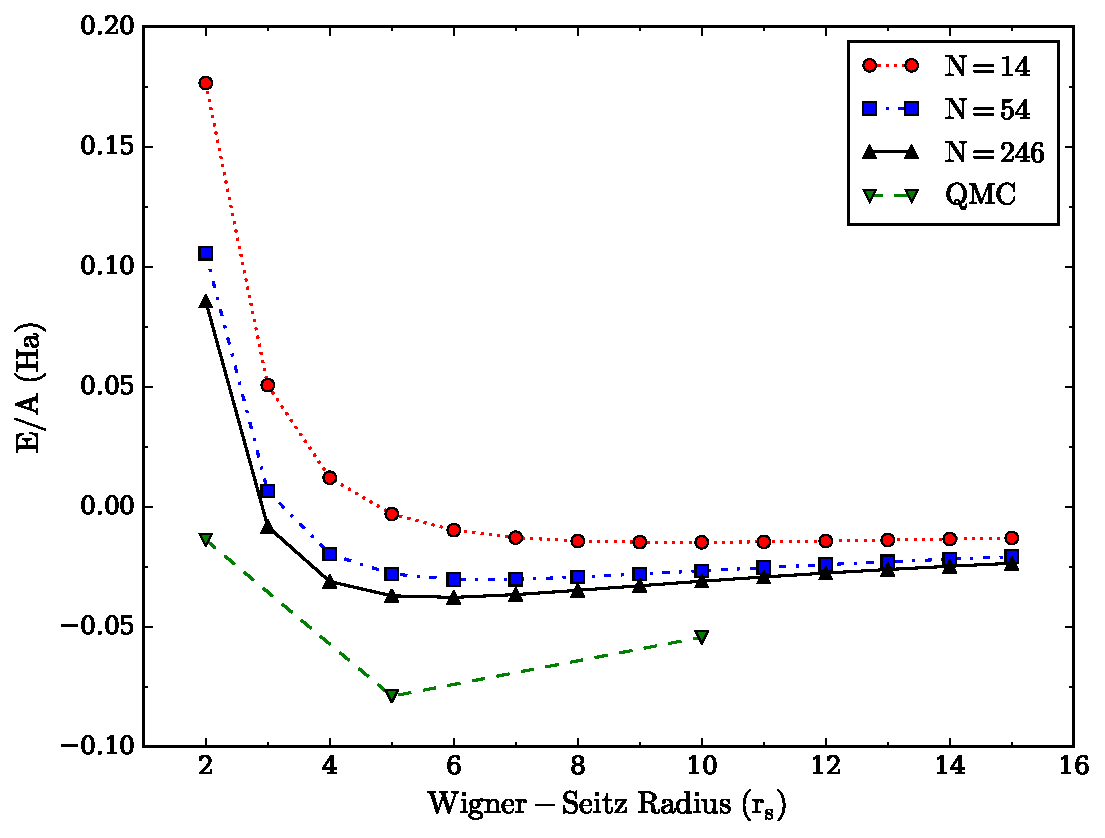
\includegraphics[width=\linewidth]{CC/Electronic_Gas.pdf}
  \caption{CCD energy per electron in Hartrees for the 3D homogeneous electron gas as function of the Wigner-Seitz radius in units of Bohr radii. The calculation used periodic boundary conditions and a basis with 25 shells, resulting in a total of $1238$ single-particle states. Also plotted are the variational quantum Monte Carlo (QMC) results from \cite{LOPEZ2006}.}  
  \label{fig:Electronic_Gas}
\end{figure}
In the limit $N,L,A \rightarrow \infty$, the plot in Fig.\ \ref{fig:Electronic_Gas} represents the equation-of-state for a 3D electron gas at absolute zero.  This curve can reveal many thermodynamic properties of the electron gas including the saturation density and saturation energy which occurs at the lowest point on the curve.  The CCD results are compared with the quasi-exact results from variational quantum Monte Carlo calculations from \cite{LOPEZ2006}.  Some of the discrepency between saturation energies from the two methods can be attributed to an insufficient basis size.  However, even an appropriate extrapolation to an infinite basis won't be able to recover all of the required correlations, which suggests that CCSDT might be able.  Regardless of the value to the saturation energy, these CCD calculations do qualitatively reproduce the saturation radius at $r_{s} \approx 5.0$.




\section{Coupled Cluster for Finite Nuclei} \label{section:cc_nuclei}

\begin{figure}[h]
  \centering
  \fbox{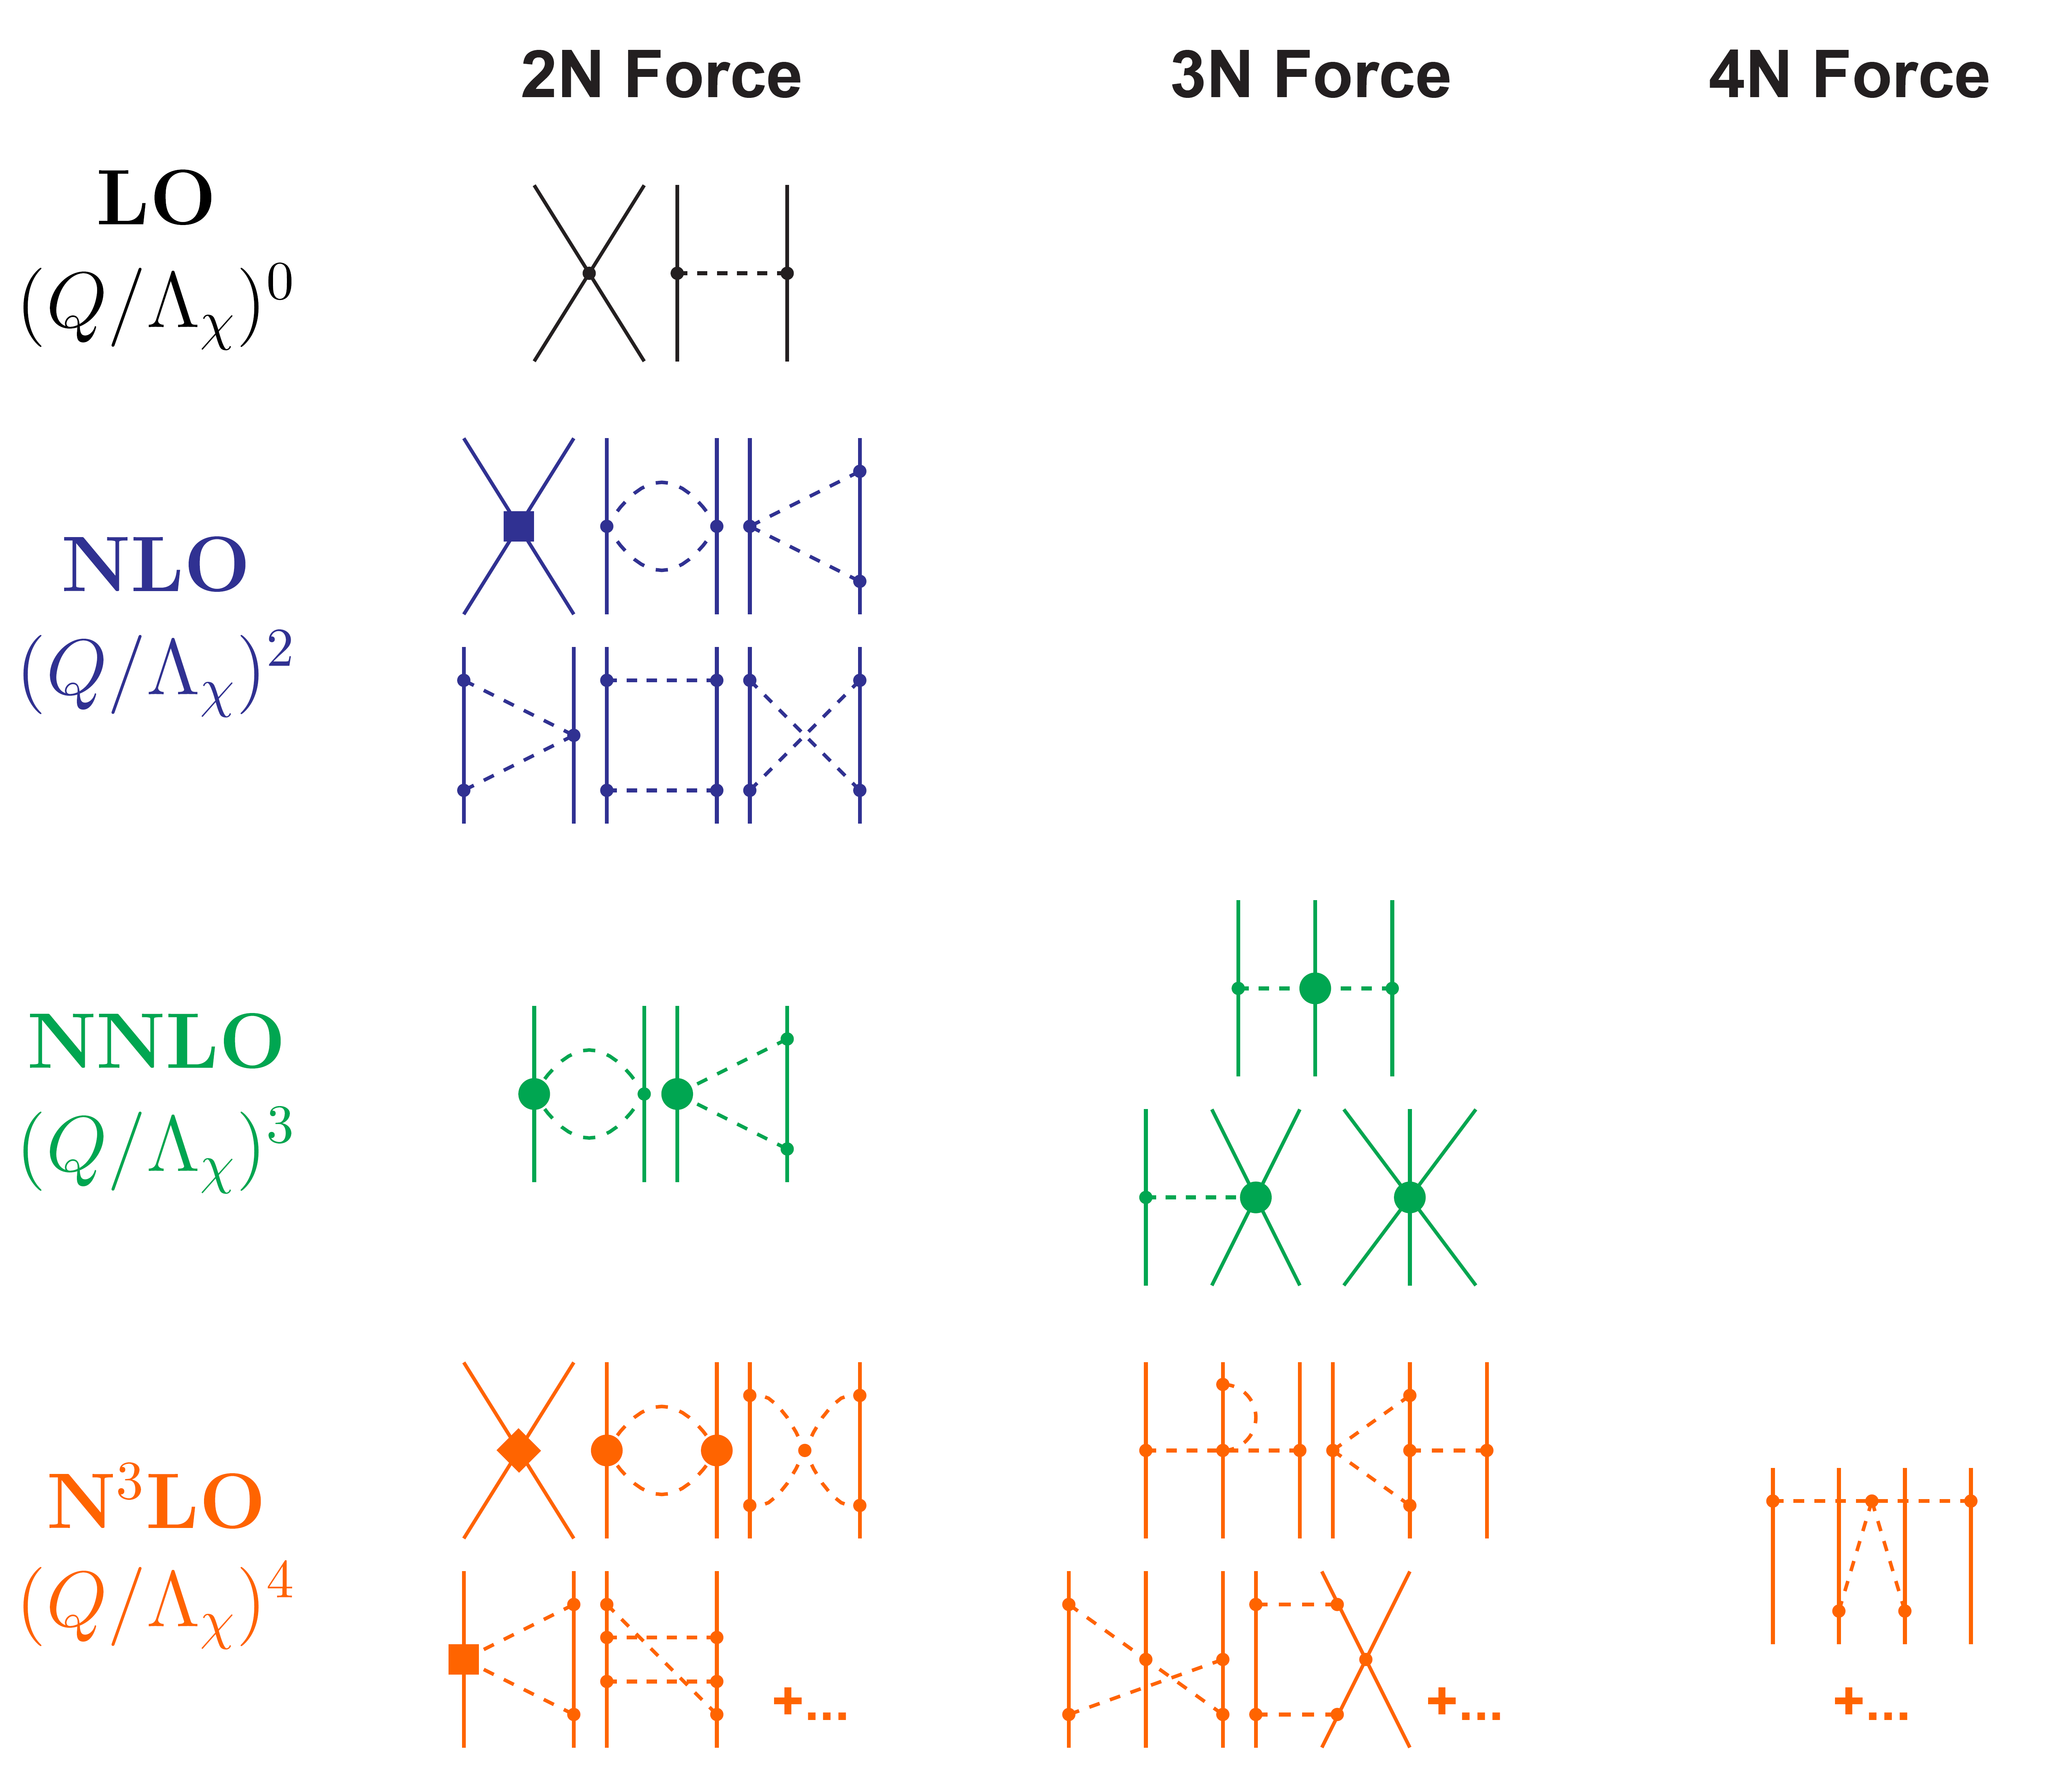
\includegraphics[width=0.7\linewidth]{CC/chiralforces.png}}
  \caption{Figure taken from \cite{MACHLEIDT2016}.}  
  \label{fig:Chiral_Forces}
\end{figure}

\begin{figure}[h]
  \centering
  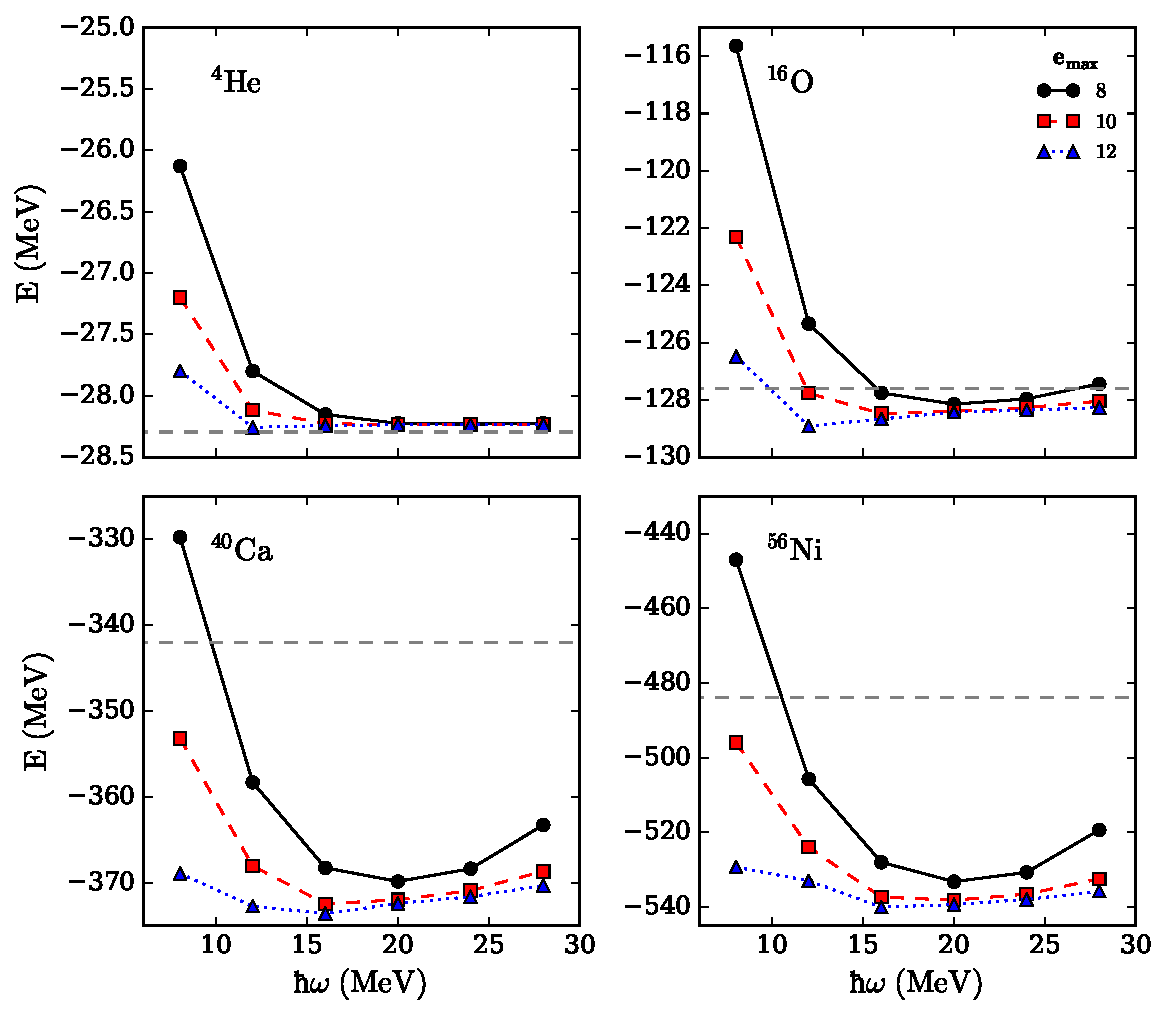
\includegraphics[width=0.85\linewidth]{CC/ground_state1.pdf}
  \caption{CCD energy per electron in Hartrees for the 3D homogeneous electron gas as function of the Wigner-Seitz radius in units of Bohr radii. The calculation used periodic boundary conditions and a basis with 25 shells, resulting in a total of $1238$ single-particle states. Also plotted are the variational quantum Monte Carlo (QMC) results from \cite{LOPEZ2006}.}  
  \label{fig:Ground_State1}
\end{figure}

\begin{figure}[h]
  \centering
  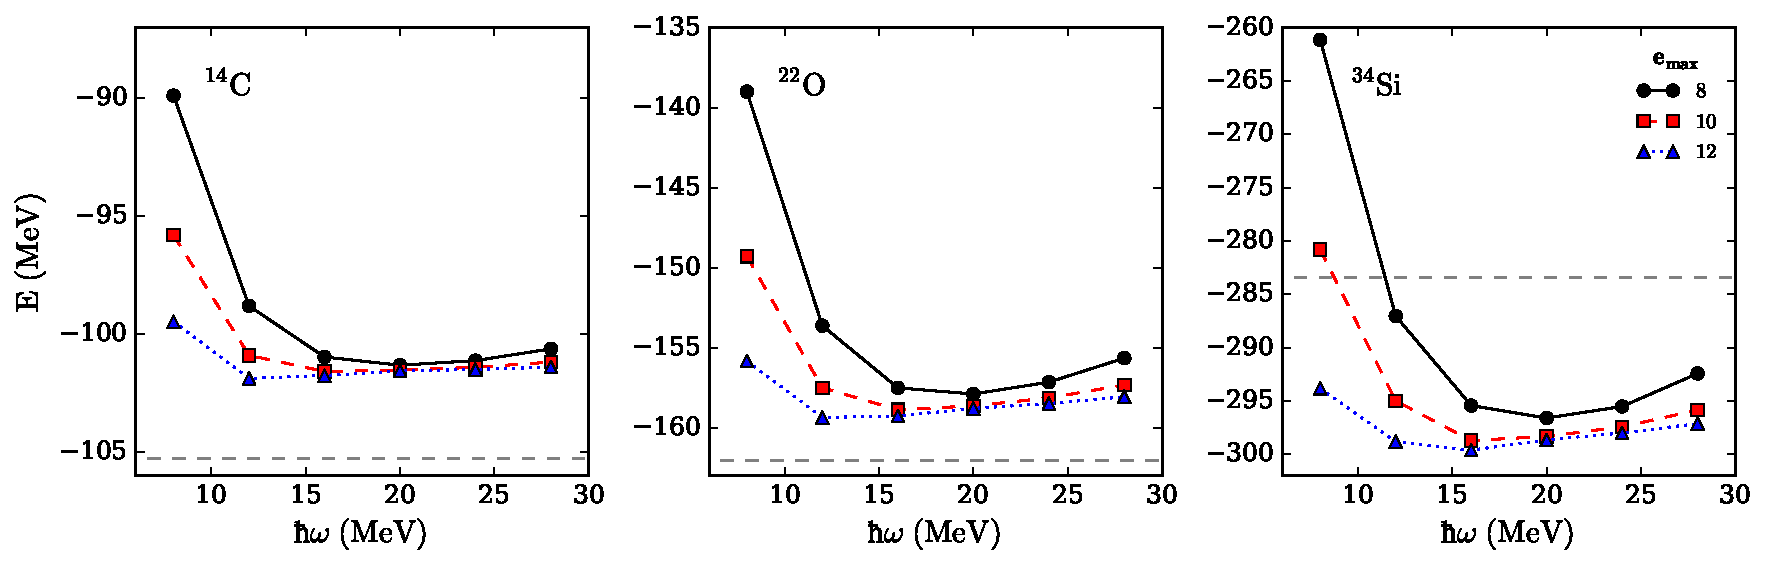
\includegraphics[width=\linewidth]{CC/ground_state2.pdf}
  \caption{CCD energy per electron in Hartrees for the 3D homogeneous electron gas as function of the Wigner-Seitz radius in units of Bohr radii. The calculation used periodic boundary conditions and a basis with 25 shells, resulting in a total of $1238$ single-particle states. Also plotted are the variational quantum Monte Carlo (QMC) results from \cite{LOPEZ2006}.}  
  \label{fig:Ground_States2}
\end{figure}


\end{document}
